There is a growing awareness of biotic interactions being crucial components of biodiversity and relevant descriptors of ecosystems \citep{valiente,jordanoS}. 
Such interactions can be conveniently represented by networks, which have been increasingly studied and used in recent years for describing and understanding living systems in ecology \citep{poisot}, microbiology \citep{faust} or genomics \citep{evans}. 
Observing species interactions is a laborious task which restricts them to certain categories (e.g.  pollination\validSR{, predation, parasitism}), while many other \validSR{types of} interactions may be hard to observe and key in the system organization (e.g. communication, shelter sharing). Many efforts have been devoted in the last decade to get a more complete picture of the biotic interactions existing between species living in the same niche: \validSR{all these interactions can be gathered in a so-called \textit{species interaction network}}.

\paragraph{Network reconstruction.} 
A first attempt consists in using observed interactions  to predict other possible links based on species traits matching \citep[see e.g.][]{OlF15,BGT16,WeG17,GrW18}. The  interaction strength can also be predicted \citep{WeO13}. This  can be viewed as a prediction task, and modern approaches arising from signal processing and machine learning have been also proposed \citep{DPL17,SPW17,DPD17}. We name these approaches {\sl network reconstruction} to distinguish them from {\sl network inference}, which is the problem we consider in this article.

\paragraph{Network inference.} 
Network inference approaches also aim at retrieving the interactions among species, but do not rely on observed interactions and therefore, remain agnostic as for their type. Such approaches have been developed in many domains ranging from cell biology \citep[][to infer gene regulatory networks]{Fri04} to neurosciences \citep[][to deciphere brain connectivity structures]{ZhC18}. In ecology, it will typically aim at inferring the set of biotic interactions linking species from the same guild.  As  summarized in Fig.~\ref{fig:networkinference}, network inference takes as input measures on species \validSR{(here abundances)} at similar sites, and returns a network of species direct interactions. The importance of distinguishing between direct interaction and indirect association between species is explained in \citet{PWT19}. 

\validSR{Species not engaged in biotic interactions can appear  linked if they respond similarly or oppositely to an abiotic effect (spurious interaction). Therefore network inference must account for environmental covariates.} Fig.~\ref{fig:graphmodel} illustrates this phenomenon: \validSR{ in ($c$) } species (1 and 4) are not in direct interaction, but are affected by the variations of the same environmental covariate $x$. ($d$) displays the network when $x$ is not accounted for: a spurious edge appears between species.


\begin{figure}[H]
    \centering
    \begin{tabular}{ccccc}
        {\tt \begin{tabular}{rr}
date & site \\
%\hline
apr93 & km03 \\
apr93 & km03 \\
apr93 & km03 \\
apr93 & km03 \\
apr93 & km17 \\
apr93 & km17 \\
\vdots & \vdots
\end{tabular} } & \qquad &
        {\tt \begin{tabular}{rrrrr}
EFI & ELA & GDE & GME & HFA \\
%\hline
 71 &   1 &   5 &   6 &   0 \\
118 &   2 &   3 &   0 &   0 \\
 69 &   0 &   6 &   2 &   0 \\
 56 &   0 &   0 &   0 &   0 \\
  0 &   1 &   1 &   0 &   0 \\
  0 &   0 &   2 &   0 &   0 \\
\vdots & \vdots & \vdots & \vdots & \vdots
\end{tabular}
%
%\begin{tabular}{rrrrrrr}
%\dots & EFI & ELA & GDE & GME & HFA & \dots \\
%\hline
%&  71 &   1 &   5 &   6 &   0 & \\
%& 118 &   2 &   3 &   0 &   0 & \\
%&  69 &   0 &   6 &   2 &   0 & \\
%&  56 &   0 &   0 &   0 &   0 & \\
%&   0 &   1 &   1 &   0 &   0 & \\
%&   0 &   0 &   2 &   0 &   0 & \\
%& \vdots & \vdots & \vdots & \vdots & \vdots
%\end{tabular} } & \qquad &
        \begin{tabular}{c}
        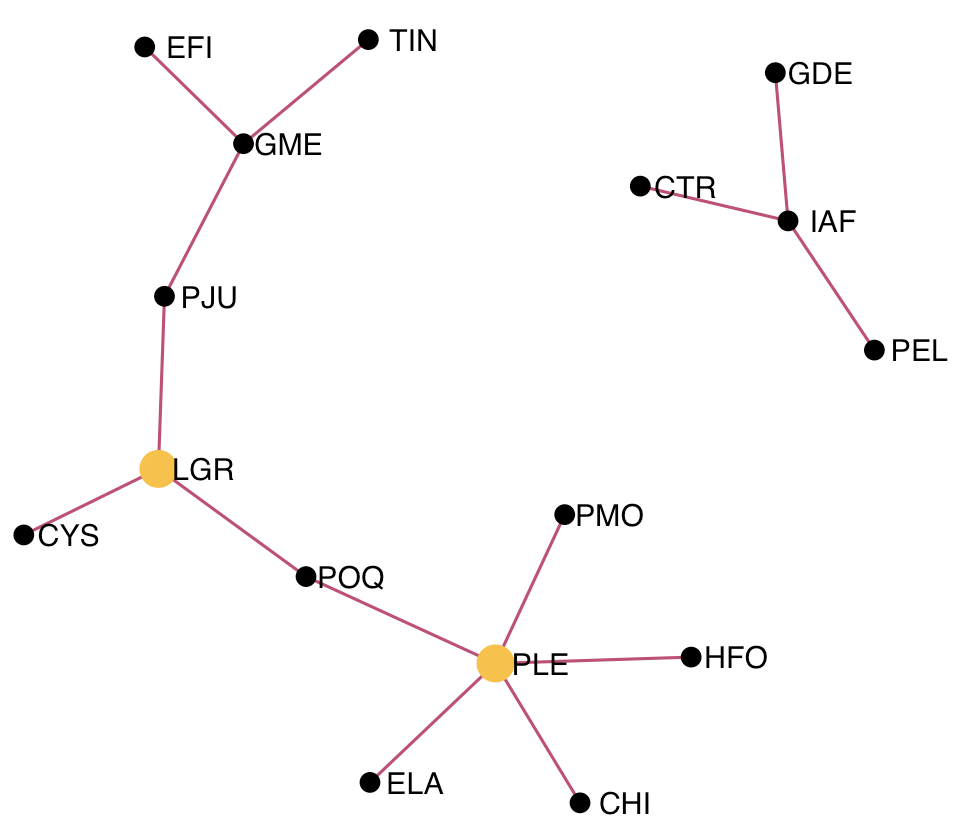
\includegraphics[width=.3\linewidth]{figs/barans2plot.png}
        \end{tabular} \\
        ($a$) covariates & & ($b$) species abundances & & ($c$) inferred network \\
    \end{tabular}
    \caption{Aim of species interaction network inference from abundance data. Data sample from the Fatala river dataset (see Section \ref{sec:datasets}). }
    \label{fig:networkinference}
\end{figure}

\paragraph{Joint species distribution models.} \validSR{ The rationale behind network inference} is that interactions between species must affect their joint distribution in a series of similar sites. 
Such approaches necessarily rely on a {\sl joint} species distribution model (JSDM), as opposed to species distribution models \citep{SDM} where species are traditionally considered as disconnected entities. 
A JSDM is a probabilistic model describing the species simultaneous presence/absence \citep{Har15,OTN17} or joint abundances \citep{PHW18,PWT19}. An important feature of JSDMs is to include environmental covariates to account for abiotic interactions. \\
Recently, latent variable models have received attention in community ecology as they provide a convenient way to model the dependence structure between species  \citep{WBO15}. The JSDM proposed by \cite{PHW18,PWT19} involves a latent layer. So does the Poisson log-Normal model \citep[PLN,][]{AiH89}, which combines generalized linear models to account for covariates and offsets, and a Gaussian latent structure to describe the species interactions. It can be seen as a multivariate mixed model, in which correlated random effects encode the dependency between the species abundances. 

\begin{figure}[H]
    \centering
    \begin{tabular}{ccccccc}
          \begin{tikzpicture}
  \node[observed] (1) at (-0.5*\edgeunit,  .5*\edgeunit) {$1$};
  \node[observed] (2) at (-0.5*\edgeunit, -.5*\edgeunit) {$2$};
  \node[observed] (3) at ( 0.5*\edgeunit, -.5*\edgeunit) {$3$};
  \node[observed] (4) at ( 0.5*\edgeunit,  .5*\edgeunit) {$4$};
  \draw[edge] (1) to (2); \draw[edge] (2) to (3); \draw[edge] (2) to (4); \draw[edge] (3) to (4); 
  \end{tikzpicture}
 & \qquad &
          \begin{tikzpicture}
  \node[observed] (1) at (-0.5*\edgeunit,  .5*\edgeunit) {$1$};
  \node[observed] (2) at (-0.5*\edgeunit, -.5*\edgeunit) {$2$};
  \node[observed] (3) at ( 0.5*\edgeunit, -.5*\edgeunit) {$3$};
  \node[observed] (4) at ( 0.5*\edgeunit,  .5*\edgeunit) {$4$};
  \draw[edge] (1) to (2); \draw[edge] (2) to (3);  \draw[edge] (1) to (3); 
  \end{tikzpicture}
 & \qquad &
          \begin{tikzpicture}
  \node[observed] (1) at (-0.5*\edgeunit,  .5*\edgeunit) {$1$};
  \node[observed] (2) at (-0.5*\edgeunit, -.5*\edgeunit) {$2$};
  \node[observed] (3) at ( 0.5*\edgeunit, -.5*\edgeunit) {$3$};
  \node[observed] (4) at ( 0.5*\edgeunit,  .5*\edgeunit) {$4$};
  \node[covariate] (x) at (0.0*\edgeunit,  .0*\edgeunit) {$x$};
  \draw[edge] (2) to (3); \draw[edge] (3) to (4); 
  \draw[edge] (x) to (1); \draw[edge] (x) to (4);
  \end{tikzpicture}
 & \qquad &
          \begin{tikzpicture}
  \node[observed] (1) at (-0.5*\edgeunit,  .5*\edgeunit) {$1$};
  \node[observed] (2) at (-0.5*\edgeunit, -.5*\edgeunit) {$2$};
  \node[observed] (3) at ( 0.5*\edgeunit, -.5*\edgeunit) {$3$};
  \node[observed] (4) at ( 0.5*\edgeunit,  .5*\edgeunit) {$4$};
  \node[covmiss] (x) at (0.0*\edgeunit,  .0*\edgeunit) {$x$};
  \draw[edge] (2) to (3); \draw[edge] (3) to (4); 
  \draw[edgemiss] (x) to (1); \draw[edgemiss] (x) to (4);
  \draw[edge] (1) to (4); 
  \end{tikzpicture}
 \\
        ($a$) connected & & ($b$) disconnected & & ($c$) with covariate & & ($d$) missing covariate 
    \end{tabular}
    \caption{Examples of graphical models. \validSR{($a$) All species are dependent, ($b$) 4 is independent from all others, ($c$)  1 and 4 are independent conditional on  $x$, ($d$) not accounting for  $x$ induces a spurious dependence between  1 and 4.}}
    \label{fig:graphmodel}
\end{figure}

\paragraph{Graphical models: a generic framework for network inference.}
Although they describe the dependence structure between the distributions of all the species from a same niche, JSDM are not sufficient to perform network inference as they do not distinguish  indirect associations from direct interactions \citep{DBD18}. Graphical models \citep{Lau96} provide a probabilistic framework to do so and, in the same time, a formal definition of the network to be inferred. This formalism is therefore especially appealing for the inference of species interaction networks \citep{PWT19}.
In an undirected graphical model \citep[which is the same as a Markov random field:][]{CWL18}, two species are connected if they are {\sl dependent} conditional on all other species, that is if the variations of their respective abundances would still be  correlated if ever both the environmental conditions and the abundances of all other species were kept fixed. Two species are unconnected if they are {\sl independent} conditional on all other species: the observed correlation between them only results from a series of links with other species \citep{morueta2016network} \validSR{or environmental effects} . 
Fig.~\ref{fig:graphmodel} illustrates the concept of conditional dependence/independence with toy graphical models. In ($a$), the network is connected so all species are interdependent: an association exists between any two of them. However, 1 is only directly interacting with 2 which mediates its association with 3 and 4: 1 is independent from them conditional on 2.

In ($b$), the network is disconnected: species 4 is independent from all others. This illustrates that graphical models enjoy all the desirable properties to represent interactions between species in an interpretable manner, so that they can be used as the mathematical counterpart of species interaction networks.

\modif{\paragraph{Network inference: the general problem.}
Network inference methods attempts to retrieve the graphical model underlying the distribution of  \review{abundance} data. In every domains, network inference is impeded by the huge number of possible graphs for a given set of nodes, which increases super-exponentially with the latter (more than $10^{13}$ undirected graphs can be drawn between 10 nodes, and more than $10^{57}$ between 20). The exploration of the graph space is therefore intractable from a combinatorial point of view. To reduce the search space, a common and reasonable assumption is that a relatively small fraction of species pairs are in direct interaction: the network is sparse. In the case of continuous observations, one of the most popular  approaches is the graphical lasso \citep[glasso:][]{GLasso} which takes advantage of the properties of Gaussian graphical models (GGM) to efficiently infer a sparse network.   
Alternatively, tree-based approaches have been proposed: \cite{ChowLiu} first made the too stringent assumption that the network is made of a single spanning tree (that is connecting all nodes without any loop, as in Fig.~\ref{fig:treeaveraging}).
More recent approaches introduced by \cite{,MeilaJaak} and \cite{kirshner} rely on efficient algebraic tools to average over all possible tree-structured graphical models. The inferred network resulting from such an averaging procedure is not restricted to be a tree: species or groups of species can be isolated (e.g. Fig.~\ref{fig:networkinference}), and loops can appear (e.g. Fig.~\ref{fig:treeaveraging}). }

\paragraph{Network inference from species abundance data.}
This work focuses on network inference based on abundance data, and not only their presence/absence \citep[as considered in][]{OHS10,CWL18}.
Network inference from species abundance measures is a notoriously difficult problem \citep{ulrich2010null}, not only because network inference is complex, but also because it has to account for the data specificities. Abundance data may spread over a wide range of values and often result from sampling efforts (sample and/or species-specific), making them difficult to compare. 
Obviously, count data do not directly fit the Gaussian framework but many network inference methods dedicated to abundance data actually rely on a latent Gaussian structure (see Section \ref{altmethods}).
 

\paragraph{Contribution.}
In the present work, we adopt a model-based approach to perform network inference from abundance data. To accommodate the data specificities we use a PLN model, which includes the over-dispersion of the observed counts as well as the sampling effort. Importantly, the PLN model \validSR{allows us} to account for abiotic effects and avoid the detection of spurious interactions between species.  \\
As for the network inference, we adopt a tree-based approach \citep[as opposed to][which also use a PLN model but resort to glasso]{MInt}, which provides a probability for each edge to be actually part of the underlying graphical model.

\paragraph{Outline.}
We introduce the method EMtree, which combines two (variational) \validSR{Expectation-Maximization (EM)} algorithms to estimate the model parameters. Importantly, our approach provides the probability for each possible edge to be part of the interaction network. We evaluate our approach on both synthetic and ecological datasets. An R package implementing EMtree is available on GitHub \url{https://github.com/Rmomal/EMtree}.  
